\documentclass[conference]{IEEEtran}
\IEEEoverridecommandlockouts
\usepackage{fontspec}\setmainfont{texgyretermes}[Extension=.otf,UprightFont=*-regular,BoldFont=*-bold,ItalicFont=*-italic,BoldItalicFont=*-bolditalic]
\usepackage{cite,amsmath,amssymb,graphicx,xcolor,tikz,booktabs,colortbl,array,eso-pic,tcolorbox}
\usetikzlibrary{svg.path,calc}
\definecolor{Cd}{HTML}{B31B1B}\definecolor{M}{HTML}{2456A6}\definecolor{Wm}{HTML}{DC6A12}\definecolor{Sm}{HTML}{14977A}\definecolor{Dfc}{HTML}{2456A6}
\definecolor{Zn}{HTML}{E9EDF6}\definecolor{Za}{HTML}{FBF1E6}\definecolor{Ze}{HTML}{F1EBF6}
\usepackage[pdftitle={Hi Is All You Need},pdfauthor={Anh Ay and Em Ay},pdfborderstyle={/S/U/W 0.6},citebordercolor={0.1 0.6 0.3},linkbordercolor={0.7 0.1 0.1},urlbordercolor={0.1 0.4 0.8}]{hyperref}
\newtcolorbox{pbox}[1]{colback=#1!7,colframe=#1!55,boxrule=.4pt,arc=1.2pt,left=3pt,right=3pt,top=2pt,bottom=2pt,before upper={\small}}
\AddToShipoutPictureBG*{\AtPageLowerLeft{\put(21,150){\rotatebox{90}{\fontsize{20}{20}\selectfont\color{gray} thínhXiv:2611.01419v1 [cs.DM] 9 Nov 2026}}}}
\begin{document}
\title{\textcolor{Cd}{``Hi'' Is All You Need: Who Texted First in 1,419 Vietnamese TikTok Couples}}
\author{\IEEEauthorblockN{Anh Ấy\textsuperscript{1,*}}\IEEEauthorblockA{\textsuperscript{1}Department of Talking Stages\\Đại học Đã Xem}\and\IEEEauthorblockN{Em Ấy\textsuperscript{2,*}}\IEEEauthorblockA{\textsuperscript{2}Institute of Applied Thả Thính\\*Equal contribution. Who contributed first is disputed.}\and\IEEEauthorblockN{Reviewer 2\textsuperscript{3}}\IEEEauthorblockA{\textsuperscript{3}Ủy ban Bao Giờ Cưới\\Standing Committee of Mothers}}
\maketitle
\begin{abstract}In two waves of a Vietnamese TikTok trend, couples posted the first messages they ever sent each other. We scanned 53,333 public posts and found 1,419 from the trend, about 58\% of an estimated 2,400, then labelled who texted first. The man did in 70\% of couples where the evidence allows a call (569 of 816; 95\% interval 66 to 73). He is also the older one 79\% of the time, and he still goes first in 58\% of couples where she is older. Women send 38\% of first messages during office hours and 14\% before 09:00. Men declare their intent about twice as often, while women more often find an excuse. Every couple in the sample got together, so this study says who started it and nothing about whose approach works.\end{abstract}
\begin{IEEEkeywords}talking stage, thả thính, first-mover disadvantage, pronoun-based age inference, survivorship bias, Reviewer 2\end{IEEEkeywords}
\section{\textcolor{Cd}{Introduction}}
Most couples keep an official account of who texted first. It tends to change depending on who is telling it and whether the other person is in the room. Mothers raise the matter at family meals \cite{me}, yet the field has no reference dataset.

Earlier work studied first contact before anyone involved had anything to lose. On a US dating site, women were 4 times less likely than men to send messages, and the women who did write connected with more desirable partners than those who waited \cite{kreager}. Across four large US cities, men and women alike pursued partners about 25\% more desirable than themselves \cite{bruch}. Field experiments have gone further and sent confederates to approach strangers directly \cite{clark}, a design our ethics board, which is one mother, declined to reproduce.

Our source is a public TikTok trend from Vietnam. In September 2026, couples began posting photo carousels of how they first started talking, usually with screenshots of the messages themselves. Two cover lines dominate the trend: ``Ủa hồi đó anh với em nhắn gì mà giờ thành đôi vậy'' (mostly September) and ``Khi bạn chỉ định nhắn tin thả thính cho vui mà mọi chuyện lại đi quá xa'' (from late October). These posts offer something reviewers often request and rarely get. The outcome is known, because the couple is together and has decided to tell everyone.

This paper makes the following contributions:

\begin{enumerate}\item A dataset of 1,419 trend posts drawn from 53,333 scanned, labelled for who sent the first message (Section II).\item The Anh Conjecture, and a test of whether it survives the woman being older (Sections III-B and III-C).\item A time zone analysis of first messages, broken down by sender (Section III-D).\item TIB-10, a taxonomy of ten opening moves grouped by how much the sender is willing to admit (Section III-F).\end{enumerate}
\section{\textcolor{Cd}{Data and Methods}}
\subsection{Collection}
We ran a logged-in, read-only browser for about 20 hours, walking the trend's sound pages and running exact-phrase searches. The crawl scanned 53,333 public posts and found 1,419 trend posts with 48.1 million plays between them. TikTok stops serving a sound after about 3,000 posts, so completeness is out of reach. The overlap between sound lists and search lists gives a capture-recapture estimate of the total, using Chapman's estimator:

\begin{equation}\hat{N}=\frac{(n_1+1)(n_2+1)}{m+1}-1\approx 2{,}400\end{equation}
Here $n_1$ and $n_2$ are the sizes of the two lists and \emph{m} is their overlap. We hold about 58\% of that total. Both methods favor the same popular posts, so the real total is probably higher.

\subsection{Labelling}
Apple's Vision OCR read the screenshots, and language-model agents labelled each post. A blind second pass agreed with the first on 44 of 45 first movers. Codex, reading 60 name-scrubbed chats independently, matched on who is older in 40 of 40 cases where both answered and on the first mover in 12 of 13. Against 10 real screenshots, first sender, true start and time matched in all 10.

\begin{pbox}{Dfc}\textbf{Definition 1 (Talking stage).} The interval that begins with the first message and ends when one party asks what this is. We do not measure its end.\end{pbox}
\begin{pbox}{Dfc}\textbf{Definition 2 (Evidence tiers).} Proof: the true start of the chat is visible, or the couple states who went first. Screen: Proof plus posts where we use the earliest message shown. Guess: Screen plus posts where the sender's gender comes from assuming who posted, using chat text or display name where possible and otherwise assuming a woman.\end{pbox}
Unless noted, we report Proof + Screen. Relative age comes from how the couple address each other (\emph{anh/em}, \emph{chị/em}). Stated ages are too rare to use, and we do not estimate ages from faces.

\section{\textcolor{Cd}{Results}}
\subsection{Who texted first}
The man sent the first message in 569 of 816 couples (70\%, Wilson 95\% interval \cite{wilson} 66 to 73). Table~\ref{tab1} shows the answer holding still as the evidence rules loosen. In the US dating data the ratio was 4 to 1 \cite{kreager}, and here it is about 2.3 to 1. The two populations differ in country, platform and outcome, so the comparison means little, and we report it anyway.

\begin{table}[t]\centering\caption{He texted first, by evidence tier}\label{tab1}\begin{tabular}{lrrr}\toprule\rowcolor{Cd!10}Tier & Couples & Man first & 95\% interval\\\midrule Proof & 585 & 72\% & 68 to 75 \\Proof + Screen & 816 & 70\% & 66 to 73 \\Proof + Screen + Guess & 1028 & 71\% & 68 to 73 \\\bottomrule\end{tabular}\end{table}
\subsection{The Anh Conjecture}
\begin{pbox}{Wm}\textbf{Observation 1 (The Anh Conjecture).} In couples whose age order can be read, the man is older in 483 of 609 cases (79\%). See Fig.~\ref{fig1}.\end{pbox}
\emph{Proof sketch.} In 483 couples, someone said \emph{anh} and meant it.

The direction agrees with a study of mate preferences across 37 samples \cite{buss}, which needed questionnaires in 33 countries where we needed the word \emph{anh}. Our estimate probably runs high, since couples can use \emph{anh/em} at the same age.

\subsection{When she is older}
\begin{pbox}{Sm}\textbf{Proposition 1.} When she is older, the man still sends the first message in 44 of 76 couples (58\%). When he is older, the figure is 336 of 471 (71\%). See Fig.~\ref{fig2}.\end{pbox}
Older women may start things a little more often. With Proof only, the gap narrows to 69\% against 72\%, on 55 older-woman couples, so we report it as a hint. Hints are a recognized opening strategy (Section III-F).

\begin{figure}[t]\centering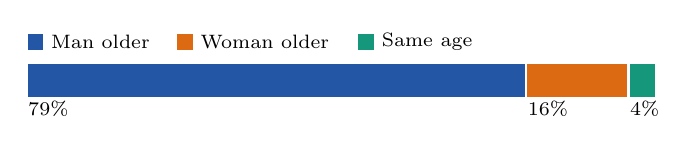
\begin{tikzpicture}\fill[M] (0,0.6) rectangle (0.2,0.8);\node[anchor=west,inner sep=2pt,font=\scriptsize] at (0.22,0.7) {Man older};\fill[Wm] (1.9,0.6) rectangle (2.1,0.8);\node[anchor=west,inner sep=2pt,font=\scriptsize] at (2.12,0.7) {Woman older};\fill[Sm] (4.199999999999999,0.6) rectangle (4.3999999999999995,0.8);\node[anchor=west,inner sep=2pt,font=\scriptsize] at (4.419999999999999,0.7) {Same age};\fill[M] (0.000,0) rectangle (6.315,0.42);\node[anchor=north west,inner sep=0,font=\scriptsize] at (0.000,-0.05) {79\%};\fill[Wm] (6.345,0) rectangle (7.615,0.42);\node[anchor=north west,inner sep=0,font=\scriptsize] at (6.345,-0.05) {16\%};\fill[Sm] (7.645,0) rectangle (7.970,0.42);\node[anchor=north west,inner sep=0,font=\scriptsize] at (7.645,-0.05) {4\%};\end{tikzpicture}\caption{He is the older one 79\% of the time. Age order read from how each couple addresses each other (609 couples).}\label{fig1}\end{figure}
\begin{figure}[t]\centering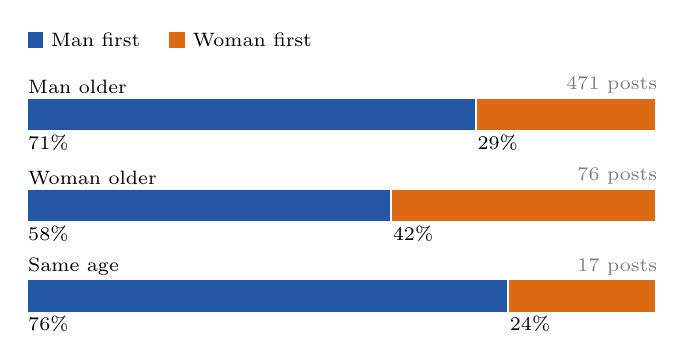
\begin{tikzpicture}\fill[M] (0,2.5) rectangle (0.2,2.7);\node[anchor=west,inner sep=2pt,font=\scriptsize] at (0.22,2.6) {Man first};\fill[Wm] (1.8,2.5) rectangle (2.0,2.7);\node[anchor=west,inner sep=2pt,font=\scriptsize] at (2.02,2.6) {Woman first};\node[anchor=south west,inner sep=0,font=\scriptsize] at (0,1.91) {Man older};\node[anchor=south east,inner sep=0,font=\scriptsize,gray] at (8,1.91) {471 posts};\fill[M] (0.000,1.45) rectangle (5.677,1.85);\node[anchor=north west,inner sep=0,font=\scriptsize] at (0.000,1.4) {71\%};\fill[Wm] (5.707,1.45) rectangle (7.970,1.85);\node[anchor=north west,inner sep=0,font=\scriptsize] at (5.707,1.4) {29\%};\node[anchor=south west,inner sep=0,font=\scriptsize] at (0,0.76) {Woman older};\node[anchor=south east,inner sep=0,font=\scriptsize,gray] at (8,0.76) {76 posts};\fill[M] (0.000,0.30000000000000004) rectangle (4.602,0.7000000000000001);\node[anchor=north west,inner sep=0,font=\scriptsize] at (0.000,0.25000000000000006) {58\%};\fill[Wm] (4.632,0.30000000000000004) rectangle (7.970,0.7000000000000001);\node[anchor=north west,inner sep=0,font=\scriptsize] at (4.632,0.25000000000000006) {42\%};\node[anchor=south west,inner sep=0,font=\scriptsize] at (0,-0.38999999999999985) {Same age};\node[anchor=south east,inner sep=0,font=\scriptsize,gray] at (8,-0.38999999999999985) {17 posts};\fill[M] (0.000,-0.8499999999999999) rectangle (6.088,-0.44999999999999984);\node[anchor=north west,inner sep=0,font=\scriptsize] at (0.000,-0.8999999999999999) {76\%};\fill[Wm] (6.118,-0.8499999999999999) rectangle (7.970,-0.44999999999999984);\node[anchor=north west,inner sep=0,font=\scriptsize] at (6.118,-0.8999999999999999) {24\%};\end{tikzpicture}\caption{Even when she is older, he usually still goes first. Share of first messages by who is older.}\label{fig2}\end{figure}
\subsection{Time zones}
We split the day into three time zones by the hour of the first message (Fig.~\ref{fig3}). In the Nocturnal Zone, from midnight to 09:00, women sent 14 of 98 first messages (14\%). In the Administrative Zone, from 09:00 to 18:00, they sent 78 of 204 (38\%). The Evening Zone sits between them at 28\%. The gap between the first two has \emph{z} = 4.2 and survives restricting to Proof (14\% against 37\%).

Volume peaks between 21:00 and midnight, which holds 31\% of all first messages in 3 of the 24 hours. No first message in the sample was sent between 04:00 and 04:59.

Reviewer 2 asked for a mechanism. We propose that a message sent during office hours can be defended as being about work. We have no evidence for this.

\begin{figure*}[t]\centering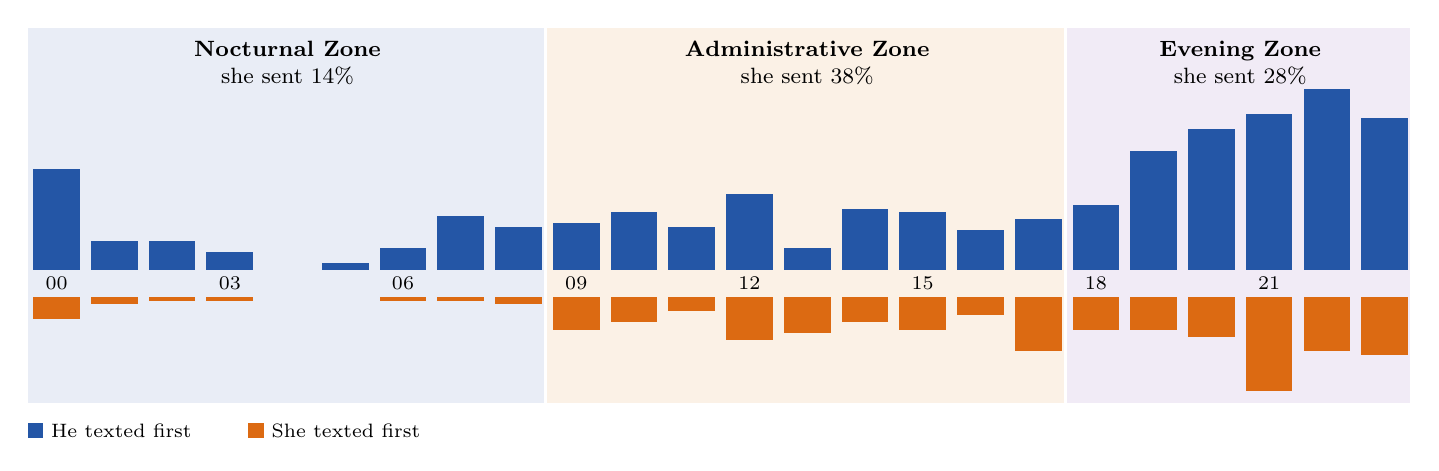
\begin{tikzpicture}\fill[Zn] (0.000,-1.516) rectangle (6.560,3.25);\node[align=center,font=\footnotesize,anchor=north] at (3.300,3.2) {\textbf{Nocturnal Zone}\\ she sent 14\%};\fill[Za] (6.600,-1.516) rectangle (13.160,3.25);\node[align=center,font=\footnotesize,anchor=north] at (9.900,3.2) {\textbf{Administrative Zone}\\ she sent 38\%};\fill[Ze] (13.200,-1.516) rectangle (17.560,3.25);\node[align=center,font=\footnotesize,anchor=north] at (15.400,3.2) {\textbf{Evening Zone}\\ she sent 28\%};\fill[M] (0.070,.17) rectangle (0.663,1.458);\fill[Wm] (0.070,-.17) rectangle (0.663,-0.446);\node[font=\scriptsize] at (0.367,0) {00};\fill[M] (0.803,.17) rectangle (1.397,0.538);\fill[Wm] (0.803,-.17) rectangle (1.397,-0.262);\fill[M] (1.537,.17) rectangle (2.130,0.538);\fill[Wm] (1.537,-.17) rectangle (2.130,-0.216);\fill[M] (2.270,.17) rectangle (2.863,0.400);\fill[Wm] (2.270,-.17) rectangle (2.863,-0.216);\node[font=\scriptsize] at (2.567,0) {03};\fill[M] (3.737,.17) rectangle (4.330,0.262);\fill[M] (4.470,.17) rectangle (5.063,0.446);\fill[Wm] (4.470,-.17) rectangle (5.063,-0.216);\node[font=\scriptsize] at (4.767,0) {06};\fill[M] (5.203,.17) rectangle (5.797,0.860);\fill[Wm] (5.203,-.17) rectangle (5.797,-0.216);\fill[M] (5.937,.17) rectangle (6.530,0.722);\fill[Wm] (5.937,-.17) rectangle (6.530,-0.262);\fill[M] (6.670,.17) rectangle (7.263,0.768);\fill[Wm] (6.670,-.17) rectangle (7.263,-0.584);\node[font=\scriptsize] at (6.967,0) {09};\fill[M] (7.403,.17) rectangle (7.997,0.906);\fill[Wm] (7.403,-.17) rectangle (7.997,-0.492);\fill[M] (8.137,.17) rectangle (8.730,0.722);\fill[Wm] (8.137,-.17) rectangle (8.730,-0.354);\fill[M] (8.870,.17) rectangle (9.463,1.136);\fill[Wm] (8.870,-.17) rectangle (9.463,-0.722);\node[font=\scriptsize] at (9.167,0) {12};\fill[M] (9.603,.17) rectangle (10.197,0.446);\fill[Wm] (9.603,-.17) rectangle (10.197,-0.630);\fill[M] (10.337,.17) rectangle (10.930,0.952);\fill[Wm] (10.337,-.17) rectangle (10.930,-0.492);\fill[M] (11.070,.17) rectangle (11.663,0.906);\fill[Wm] (11.070,-.17) rectangle (11.663,-0.584);\node[font=\scriptsize] at (11.367,0) {15};\fill[M] (11.803,.17) rectangle (12.397,0.676);\fill[Wm] (11.803,-.17) rectangle (12.397,-0.400);\fill[M] (12.537,.17) rectangle (13.130,0.814);\fill[Wm] (12.537,-.17) rectangle (13.130,-0.860);\fill[M] (13.270,.17) rectangle (13.863,0.998);\fill[Wm] (13.270,-.17) rectangle (13.863,-0.584);\node[font=\scriptsize] at (13.567,0) {18};\fill[M] (14.003,.17) rectangle (14.597,1.688);\fill[Wm] (14.003,-.17) rectangle (14.597,-0.584);\fill[M] (14.737,.17) rectangle (15.330,1.964);\fill[Wm] (14.737,-.17) rectangle (15.330,-0.676);\fill[M] (15.470,.17) rectangle (16.063,2.148);\fill[Wm] (15.470,-.17) rectangle (16.063,-1.366);\node[font=\scriptsize] at (15.767,0) {21};\fill[M] (16.203,.17) rectangle (16.797,2.470);\fill[Wm] (16.203,-.17) rectangle (16.797,-0.860);\fill[M] (16.937,.17) rectangle (17.530,2.102);\fill[Wm] (16.937,-.17) rectangle (17.530,-0.906);\fill[M] (0,-1.9659999999999997) rectangle (0.2,-1.7659999999999998);\node[anchor=west,inner sep=2pt,font=\scriptsize] at (0.22,-1.8659999999999997) {He texted first};\fill[Wm] (2.8,-1.9659999999999997) rectangle (3.0,-1.7659999999999998);\node[anchor=west,inner sep=2pt,font=\scriptsize] at (3.02,-1.8659999999999997) {She texted first};\end{tikzpicture}\caption{First messages by hour and sender, Proof + Screen. Bars above the axis are couples where he texted first, bars below are couples where she did, on the same scale. Vietnam time.}\label{fig3}\end{figure*}
\subsection{How it opened, and where}
Messenger carries 652 of the 796 conversations with an identifiable platform (82\%). Zalo, home of the family group chat, has 75. The most common opening is a reply to a story (192 posts): someone broadcasts to all their friends and one friend takes it personally. Plain greetings come second at 188 (Fig.~\ref{fig4}). The opening type is our weakest label, matching our check on 22 of 29 posts.

\begin{figure*}[t]\centering\begin{tikzpicture}\node[anchor=west,font=\small\bfseries] at (0,.55) {(a) How it opened};\node[anchor=west,font=\small\bfseries] at (9.4,.55) {(b) Platform};\node[anchor=east,font=\footnotesize] at (2.0,0) {Story reply};\fill[Cd] (2.1,-0.14) rectangle (7.100,0.14);\node[anchor=west,font=\scriptsize] at (7.150,0) {192};\node[anchor=east,font=\footnotesize] at (2.0,-0.55) {Greeting};\fill[Cd] (2.1,-0.6900000000000001) rectangle (6.996,-0.41000000000000003);\node[anchor=west,font=\scriptsize] at (7.046,-0.55) {188};\node[anchor=east,font=\footnotesize] at (2.0,-1.1) {Question};\fill[Cd] (2.1,-1.2400000000000002) rectangle (5.616,-0.9600000000000001);\node[anchor=west,font=\scriptsize] at (5.666,-1.1) {135};\node[anchor=east,font=\footnotesize] at (2.0,-1.6500000000000001) {Flirty joke};\fill[Cd] (2.1,-1.79) rectangle (3.741,-1.5100000000000002);\node[anchor=west,font=\scriptsize] at (3.791,-1.6500000000000001) {63};\node[anchor=east,font=\footnotesize] at (2.0,-2.2) {Compliment};\fill[Cd] (2.1,-2.3400000000000003) rectangle (2.647,-2.06);\node[anchor=west,font=\scriptsize] at (2.697,-2.2) {21};\node[anchor=east,font=\footnotesize] at (2.0,-2.75) {Other};\fill[Cd] (2.1,-2.89) rectangle (5.616,-2.61);\node[anchor=west,font=\scriptsize] at (5.666,-2.75) {135};\node[anchor=west,inner sep=0] at (9.4,0) {
\includegraphics[width=.36cm]{icon_messenger.pdf}};\node[anchor=west,font=\footnotesize] at (9.85,0) {Messenger};\fill[Cd] (11.600000000000001,-0.14) rectangle (16.200,0.14);\node[anchor=west,font=\scriptsize] at (16.250,0) {652};\node[anchor=west,inner sep=0] at (9.4,-0.55) {
\includegraphics[width=.36cm]{icon_zalo.pdf}};\node[anchor=west,font=\footnotesize] at (9.85,-0.55) {Zalo};\fill[Cd] (11.600000000000001,-0.6900000000000001) rectangle (12.129,-0.41000000000000003);\node[anchor=west,font=\scriptsize] at (12.179,-0.55) {75};\node[anchor=west,inner sep=0] at (9.4,-1.1) {
\includegraphics[width=.36cm]{icon_tiktok.pdf}};\node[anchor=west,font=\footnotesize] at (9.85,-1.1) {TikTok};\fill[Cd] (11.600000000000001,-1.2400000000000002) rectangle (11.798,-0.9600000000000001);\node[anchor=west,font=\scriptsize] at (11.848,-1.1) {28};\node[anchor=west,inner sep=0] at (9.4,-1.6500000000000001) {
\includegraphics[width=.36cm]{icon_instagram.pdf}};\node[anchor=west,font=\footnotesize] at (9.85,-1.6500000000000001) {Instagram};\fill[Cd] (11.600000000000001,-1.79) rectangle (11.727,-1.5100000000000002);\node[anchor=west,font=\scriptsize] at (11.777,-1.6500000000000001) {18};\node[anchor=west,inner sep=0] at (9.4,-2.2) {
\includegraphics[width=.36cm]{icon_other.pdf}};\node[anchor=west,font=\footnotesize] at (9.85,-2.2) {Other};\fill[Cd] (11.600000000000001,-2.3400000000000003) rectangle (11.762,-2.06);\node[anchor=west,font=\scriptsize] at (11.812,-2.2) {23};\end{tikzpicture}\caption{(a) How the conversation opened. (b) The platform it happened on.}\label{fig4}\end{figure*}
\subsection{TIB-10: the Taxonomy of Initiation Behaviours}
We tagged 960 openers into ten styles without telling the tagger who sent each one. A blind re-tag of 100 agreed on 90. Fig.~\ref{fig5} groups the styles into three families according to how much the sender admits to wanting something.

\begin{pbox}{Sm}\textbf{Proposition 2 (Asymmetric Declaration).} Men open with declared intent in 91 of 537 openers (17\%). Women do so in 18 of 226 (8\%).\end{pbox}
Women lean on excuses instead, at 16.8\% against 9.5\% for men. In couples where he is older, the gap grows to 24.4\% against 8.8\%. Compliments split hardest, at 6.5\% of male openers and 0.9\% of female ones. Across all 960 openers, the word \emph{xinh} appears in 23 from men and none from women. Vietnamese has a phrase for telling a man he is handsome, \emph{đẹp trai}, and nobody used it.

We formed the families after seeing the tags. With ten styles compared, gaps under about 5 points may be chance.

\begin{figure*}[t]\centering\begin{tikzpicture}\draw[gray!25] (6.100,.25) -- (6.100,-5.769999999999999);\node[font=\scriptsize,gray] at (6.100,-5.969999999999999) {0\%};\draw[gray!25] (8.400,.25) -- (8.400,-5.769999999999999);\node[font=\scriptsize,gray] at (8.400,-5.969999999999999) {5\%};\draw[gray!25] (10.700,.25) -- (10.700,-5.769999999999999);\node[font=\scriptsize,gray] at (10.700,-5.969999999999999) {10\%};\draw[gray!25] (13.000,.25) -- (13.000,-5.769999999999999);\node[font=\scriptsize,gray] at (13.000,-5.969999999999999) {15\%};\draw[gray!25] (15.300,.25) -- (15.300,-5.769999999999999);\node[font=\scriptsize,gray] at (15.300,-5.969999999999999) {20\%};\fill[Cd!10] (0,-0.2) rectangle (17.5,0.24);\node[anchor=west,font=\footnotesize\bfseries,text=Cd] at (0,0) {Declared intent};\node[anchor=west,font=\scriptsize\itshape] at (3.4,0) {The sender admits to wanting something.};\node[anchor=east,font=\scriptsize] at (17.4,0) {men 17\%, women 8\%};\node[anchor=west,font=\footnotesize] at (0,-0.5) {Compliment};\node[anchor=west,font=\scriptsize\itshape,gray] at (2.9,-0.5) {``Ảnh đẹp thế''};\draw[gray!55,line width=1pt] (9.098,-0.5) -- (6.507,-0.5);\fill[M] (9.098,-0.5) circle (.085);\fill[Wm] (6.507,-0.5) circle (.085);\node[anchor=east,font=\scriptsize] at (17.4,-0.5) {men +5.6};\node[anchor=west,font=\footnotesize] at (0,-0.97) {Open flirting};\node[anchor=west,font=\scriptsize\itshape,gray] at (2.9,-0.97) {``Thích bạn rồi đó''};\draw[gray!55,line width=1pt] (8.927,-0.97) -- (7.321,-0.97);\fill[M] (8.927,-0.97) circle (.085);\fill[Wm] (7.321,-0.97) circle (.085);\node[anchor=east,font=\scriptsize] at (17.4,-0.97) {men +3.5};\node[anchor=west,font=\footnotesize] at (0,-1.44) {Asks to get to know};\node[anchor=west,font=\scriptsize\itshape,gray] at (2.9,-1.44) {``Làm quen nhé''};\draw[gray!55,line width=1pt] (8.070,-1.44) -- (8.135,-1.44);\fill[M] (8.070,-1.44) circle (.085);\fill[Wm] (8.135,-1.44) circle (.085);\node[anchor=east,font=\scriptsize] at (17.4,-1.44) {women +0.1};\fill[Cd!10] (0,-2.19) rectangle (17.5,-1.75);\node[anchor=west,font=\footnotesize\bfseries,text=Cd] at (0,-1.99) {Plausible deniability};\node[anchor=west,font=\scriptsize\itshape] at (3.4,-1.99) {The sender has a reason to be there.};\node[anchor=east,font=\scriptsize] at (17.4,-1.99) {men 25\%, women 30\%};\node[anchor=west,font=\footnotesize] at (0,-2.49) {Finds an excuse};\node[anchor=west,font=\scriptsize\itshape,gray] at (2.9,-2.49) {``Cho mình hỏi bài này''};\draw[gray!55,line width=1pt] (10.469,-2.49) -- (13.835,-2.49);\fill[M] (10.469,-2.49) circle (.085);\fill[Wm] (13.835,-2.49) circle (.085);\node[anchor=east,font=\scriptsize] at (17.4,-2.49) {women +7.3};\node[anchor=west,font=\footnotesize] at (0,-2.96) {Shared link};\node[anchor=west,font=\scriptsize\itshape,gray] at (2.9,-2.96) {``Bạn của X phải không''};\draw[gray!55,line width=1pt] (9.698,-2.96) -- (8.746,-2.96);\fill[M] (9.698,-2.96) circle (.085);\fill[Wm] (8.746,-2.96) circle (.085);\node[anchor=east,font=\scriptsize] at (17.4,-2.96) {men +2.1};\node[anchor=west,font=\footnotesize] at (0,-3.4299999999999997) {Reacts to a story};\node[anchor=west,font=\scriptsize\itshape,gray] at (2.9,-3.4299999999999997) {``Đi đâu vậy''};\draw[gray!55,line width=1pt] (9.526,-3.4299999999999997) -- (9.357,-3.4299999999999997);\fill[M] (9.526,-3.4299999999999997) circle (.085);\fill[Wm] (9.357,-3.4299999999999997) circle (.085);\node[anchor=east,font=\scriptsize] at (17.4,-3.4299999999999997) {men +0.4};\fill[Cd!10] (0,-4.18) rectangle (17.5,-3.7399999999999993);\node[anchor=west,font=\footnotesize\bfseries,text=Cd] at (0,-3.9799999999999995) {Small talk};\node[anchor=west,font=\scriptsize\itshape] at (3.4,-3.9799999999999995) {Nothing has been admitted yet.};\node[anchor=east,font=\scriptsize] at (17.4,-3.9799999999999995) {men 42\%, women 39\%};\node[anchor=west,font=\footnotesize] at (0,-4.4799999999999995) {Everyday question};\node[anchor=west,font=\scriptsize\itshape,gray] at (2.9,-4.4799999999999995) {``Ăn cơm chưa''};\draw[gray!55,line width=1pt] (12.696,-4.4799999999999995) -- (9.967,-4.4799999999999995);\fill[M] (12.696,-4.4799999999999995) circle (.085);\fill[Wm] (9.967,-4.4799999999999995) circle (.085);\node[anchor=east,font=\scriptsize] at (17.4,-4.4799999999999995) {men +5.9};\node[anchor=west,font=\footnotesize] at (0,-4.949999999999999) {Teases or jokes};\node[anchor=west,font=\scriptsize\itshape,gray] at (2.9,-4.949999999999999) {``Cười gì dữ vậy''};\draw[gray!55,line width=1pt] (13.553,-4.949999999999999) -- (14.852,-4.949999999999999);\fill[M] (13.553,-4.949999999999999) circle (.085);\fill[Wm] (14.852,-4.949999999999999) circle (.085);\node[anchor=east,font=\scriptsize] at (17.4,-4.949999999999999) {women +2.8};\node[anchor=west,font=\footnotesize] at (0,-5.419999999999999) {Just hi};\node[anchor=west,font=\scriptsize\itshape,gray] at (2.9,-5.419999999999999) {``Hi''};\draw[gray!55,line width=1pt] (11.325,-5.419999999999999) -- (11.392,-5.419999999999999);\fill[M] (11.325,-5.419999999999999) circle (.085);\fill[Wm] (11.392,-5.419999999999999) circle (.085);\node[anchor=east,font=\scriptsize] at (17.4,-5.419999999999999) {women +0.1};\fill[M] (0,-6.019999999999999) circle (.085);\node[anchor=west,font=\scriptsize] at (.12,-6.019999999999999) {Men's openers};\fill[Wm] (2.2,-6.019999999999999) circle (.085);\node[anchor=west,font=\scriptsize] at (2.32,-6.019999999999999) {Women's openers};\end{tikzpicture}\caption{TIB-10, Proof + Screen. Share of each sender's openers in each style, grouped by family. 537 openers from men and 226 from women. Examples are invented in the same style. The remaining openers fall under Other and are not shown.}\label{fig5}\end{figure*}
\section{\textcolor{Cd}{Threats to Validity}}
Survivorship is total. The sample contains only talking stages that worked out and got posted, so we cannot estimate anyone's success rate, and every unanswered ``hi'' is missing. We ask readers to remember this before trying anything.

Posters are not a random draw. Where gender is clear from the post, 91\% are women (691 of 758), and ``he chased me'' may simply be the better story to post. Couples also choose which screenshots to show, and 370 posts show only photos or a caption.

We ran about 60 comparisons for Table~\ref{tab2}, so some of its small-count results will be flukes.

\section{\textcolor{Cd}{Conclusion}}
Men sent about 70\% of first messages in this sample, and he still went first in most couples where she is older. Women's share of first messages peaks in office hours, and their openers rely more on excuses. The most repeated exact opener in the data is ``hi'', used by 7 couples. We do not recommend it. We can only report that it failed to prevent 7 relationships. The title follows a convention in machine learning \cite{vaswani} and is not a finding.

\begin{table}[t]\centering\caption{Findings no reviewer requested}\label{tab2}\footnotesize\begin{tabular}{p{5.0cm}p{2.9cm}}\toprule\rowcolor{Cd!10}Finding & Value\\\midrule Openers containing ``xinh'', men / women & 23 / 0\\Openers containing ``đẹp'', men / women & 21 / 1\\Openers containing ``ơi'', men / women & 4.0\% / 9.0\%\\Median likes, she went first / he went first & 92 / 65\\She went first: caption-only claims / chat on screen & 42\% / 27\%\\Rude openers, men / women & 4 / 6\\Median opener length, men / women & 22 / 21 characters\\Founding excuse: homework & 8 openers\\Founding excuse: TikTok streak & 7 (6 from women)\\Founding excuse: borrowing phone credit & 4 openers\\Founding excuse: asking for a bank number & 4 openers\\Married within 7 months of the first text & 7 of 43\\Longest first text to wedding & 10 years\\Chats containing ``:))'' & 24\%\\Rejected: men post more when she chased, all tiers / Proof & 41\% vs 28\% / 28\% vs 28\%\\\bottomrule\end{tabular}\end{table}
\section*{\textcolor{Cd}{Acknowledgment}}
Labels came from Claude sub-agents and one Codex run. No grant funded this work. The format is a parody: the counts are real, the authors, affiliations and preprint server are invented, and nobody has peer reviewed any of it.

\section*{\textcolor{Cd}{Data Availability}}
Row-level data stay private. These couples posted for their friends and did not sign up to be a dataset, so this paper reports counts only, and the example openers in Fig.~\ref{fig5} are made up.

\bibliographystyle{ieeetr}\bibliography{ref}
\end{document}
